\section{Quantum Gates}\newline


In der klassischen Informationstechnik werden logische Schaltungen mithilfe verschiedener \textit{Gates} realisiert. Ein \textit{Gate} setzt boolsche Funktionen um, die binäre Eingangssignale zu einem binären Ausgangssignal verarbeiten. \newline

Das Prinzip von Quantum Gates ist dasselbe. Häufig sind die inneren Funktionen aber deutlich komplexer, um Gebrauch von den Möglichkeiten der Quantenmechanik zu machen. \newline
\newline
\subsection{Single Qubit Gates} \newline

Um den Zustand eines einzelnen Qubits zu ändern, ohne dessen potenzielle Superposition zu zerstören, können \textit{Single Qubit Gates} auf das Qubit angewandt werden. Beispielhaft dafür sind die \textit{Pauli Gates} X, Y, und Z mit den Funktionen (Matrizen):

\begin{equation}
    X = \begin{bmatrix} 0 & 1 \\ 1 & 0 \end{bmatrix},\quad Y = \begin{bmatrix} 0 & -i \\ i & 0 \end{bmatrix},\quad Z = \begin{bmatrix} 1 & 0 \\ 0 & -1 \end{bmatrix}.
\end{equation}

Diese Single Qubit Gates führen Rotationen mit dem Wert \(\pi\) um die jeweilige Achse der Bloch Sphere durch. Liegt die Basis eines Qubits beispielsweise auf der Z-Achse mit den Eigenzuständen \(\Ket{0}\) und \(\Ket{1}\), was standardmäßig der Fall ist, so hat ein \textit{X-Gate} dieselbe Wirkung wie ein \textit{NOT-Gate} in der Digitaltechnik:

\[X\Ket{0} = \begin{bmatrix}0 & 1 \\ 1 & 0\end{bmatrix} \begin{bmatrix}1\\0\end{bmatrix} = \begin{bmatrix}0\\1\end{bmatrix} = \Ket{1}\]
Eine weitere häufig verwendete Basis ist die X-Basis, deren Eigenzustände\(\Ket{+}\) und \(\Ket{-}\) sind. Ein Umschwung von der Z-Basis auf die X-Basis kann durch das \textit{Hadamard Gate} erreicht werden.

\begin{equation}
    H = \frac{1}{\sqrt{2}} \begin{bmatrix}
        1 & 1 \\ 1 & -1
    \end{bmatrix}\end{equation}
Die Anwendung des \textit{Hadarmad Gates} auf \(\Ket{0}\) oder \(\Ket{1}\) resultiert in einer Superposition:

\begin{align*}
    H\Ket{0} & = \frac{1}{\sqrt{2}} (\Ket{0} + \Ket{1}) = \Ket{+}  \\
    H\Ket{1} & = \frac{1}{\sqrt{2}} (\Ket{0} - \Ket{1}) = \Ket{-}.
\end{align*}

Die Anwendung eines Hadarmad Gates auf ein Qubit mit dem Zustand \(\Ket{z}\) kann dank der Euler'schen Identität auch generalisiert geschrieben werden:

\begin{gather*}
    e^{x i} = cos(x) + i sin(x) \quad\xrightarrow{x=\pi}\quad e^{\pi i} = -1 \\
    H\Ket{z} = \frac{1}{\sqrt{2}} (\Ket{0} + e^{\frac{2\pi iz}{2}}\Ket{1}) = \frac{1}{\sqrt{2}} (\Ket{0} + e^{\pi iz}\Ket{1}).
\end{gather*}

Qubit Gates können hintereinander ausgeführt werden, um bestimmte logische Operationen durchzuführen. So kann die Wirkung eines \textit{X-Gates} beispielsweise auch durch zwei \textit{Hadamard Gates} und ein \textit{Z-Gate} erzielt werden:

\[
    HZH = \frac{1}{\sqrt{2}} \begin{bmatrix}
        1 & 1 \\ 1 & -1
    \end{bmatrix} \begin{bmatrix} 1 & 0 \\ 0 & -1 \end{bmatrix} \frac{1}{\sqrt{2}} \begin{bmatrix}
        1 & 1 \\ 1 & -1
    \end{bmatrix} = \begin{bmatrix} 0 & 1 \\ 1 & 0 \end{bmatrix} = X
\]

\begin{figure}
    \centering
    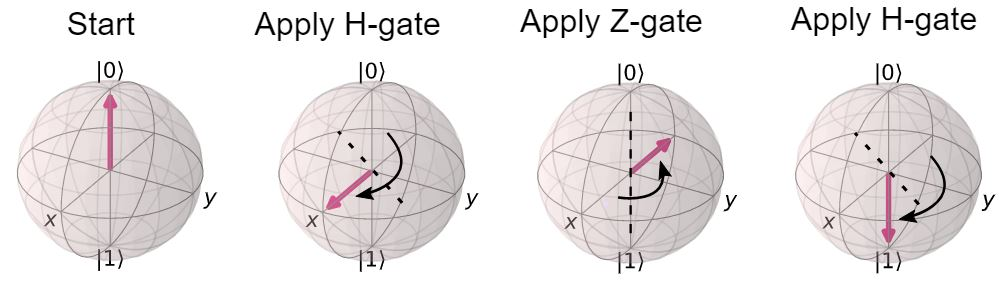
\includegraphics[width=80]{content/HZH_gate_operation.JPG}
    \caption{Visualisierung einer \(HZH\) Gatefolge auf ein Qubit mit dem Startzustand \(\Ket{0}\). 
    Nach Anwendung der Gates befindet sich das Qubit im Zustand \(1\) - es wurde ein \(X-Gate\) bzw. 
    eine \(NOT\) Operation durchgeführt. (ANIS u. a., 2021, Vgl. Textbook ’Single Qubit Gates’ - Chapter 4)}
\end{figure} \newline
\subsubsection{HZH-Gatefolge auf ein Qubit}
\circuit[name=circuit1,inline=true,editable=false,results=true]{content/circuit1.js}
\newline

Theoretisch existieren unendlich viele \textit{Singe Qubit Gates}. Dabei werden die Rotationen häufig auch parametrisiert. Die einzige Bedingung für ein valides Quantum Gate ist \textit{Unitarität}. Eine Quantum Gate \textit{U} muss also reversibel sein. Für \textit{U} bedeutet das, dass \(U^\dagger U = I\), also adjunkte Matrix \({U^\dagger}\) mal Matrix \textit{U} gleich Einheitsmatrix \textit{I}, ist.
\newline
Ein arbiträres (willkürliches) Single Qubit Gate \(U\) kann durch eine endliche Anzahl an Qubit Gates realisiert werden:

\begin{equation}\begin{gathered}

        U = e^{i\alpha} \begin{bmatrix}
            e^{-i\beta/2} & 0            \\
            0             & e^{i\beta/2}
        \end{bmatrix} \begin{bmatrix}
            \cos \frac{\gamma}{2} & -\sin \frac{\gamma}{2} \\
            \sin \frac{\gamma}{2} & \cos \frac{\gamma}{2}
        \end{bmatrix},
        \begin{bmatrix}
            e^{-i\delta/2} & 0             \\
            0              & e^{i\delta/2}
        \end{bmatrix}
        \\ \alpha, \beta, \gamma \delta \in \mathbb{R}.
    \end{gathered}\end{equation}


\glqqBeachten Sie, dass die zweite Matrix nur eine gewöhnliche Drehung ist. Es stellt sich heraus, dass die erste und die letzte Matrix auch als Drehungen in einer anderen Ebene verstanden werden können. Diese Zerlegung kann verwendet werden, um ein genaues Rezept für die Ausführung eines beliebigen Quantenlogik-Gatters auf ein einzelnes Qubit zu erhalten.\grqq (Nielsen und Chuang, 2001, S. 20)

\newline \newline
\exercise[type=multipleChoice]{
    \question{Frage: In welchem Zustand befindet sich ein Qubit, nachdem auf den Startzustand \(\Ket{0}\) eine \(HZZ\) Gatefolge angewandt wurde?}
    \possibleAnswers{
        \item 1) In Zustand \(HZZ\Ket{0} =\Ket{0}\), denn die Z Gatter funktionieren nicht hintereinander.
        \item 2) In Zustand \(HZZ\Ket{0} =\Ket{1}\).
        \item 3) In Zustand \(HZZ\Ket{0} = \frac{1}{\sqrt{2}} (\Ket{0} + \Ket{1})\), denn zwei Z Gatter hintereinander rotieren um 360° um die Z-Achse und haben somit keine Wirkung.
    }
    \result{3}
}



\newline \newline
\subsection{Multiple Qubit Gates} \newline

Obwohl es unendlich viele verschiedene Single Qubit Gates gibt, sind die Grenzen an Möglichkeiten sehr eingeschränkt. 
Multiple Qubit Gates verschaffen Abhilfe, indem komplexere Funktionen mit mehreren Qubits gleichzeitig durchgeführt werden. \newline
Auch für Multiple Qubit Gates gilt die Regel, dass die Gates unitär sein müssen. Das bedeutet, dass klassische \textit{XOR-} oder \textit{NAND-Gates} in der Welt des Quantum Computings nicht existieren und aufwändig aus anderen Gate-Kombinationen kreiert werden müssen, da diese in ihrer Natur nicht reversibel sind und dadurch Informationen verloren gehen. \newline \newline

Ein wichtiges Multiple Qubit Gate ist das \textit{Controlled NOT-Gate}. Aus \textit{CNOT-Gates} und Single Qubit Gates kann jedes beliebige Multiple Quantum Gate erstellt werden. (Nielsen und Chuang, 2001, Vgl. S.22) \newline

Ein CNOT-Gate besteht aus zwei Qubits: dem Control- und dem Target-Qubit. Ist das Control-Qubit im Zustand \(\Ket{1}\), so wird ein \textit{X-Gate} auf das Target Qubit ausgeführt. Ist das Control-Qubit \(\Ket{0}\), so verändert sich nichts.

\begin{figure}
    \centering
    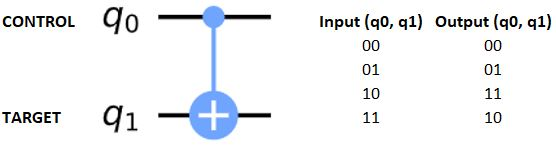
\includegraphics[width=70]{content/CNOT.JPG}
    \caption{Controlled NOT-Gate}
    \label{fig:cnot}
\end{figure}

\begin{equation}
    CNOT = \begin{bmatrix} 1 & 0 & 0 & 0 \\ 0 & 0 & 0 & 1 \\ 0 & 0 & 1 & 0 \\ 0 & 1 & 0 & 0 \\  \end{bmatrix}, \quad
    CNOT\Ket{\alpha} = \begin{bmatrix} 1 & 0 & 0 & 0 \\ 0 & 0 & 0 & 1 \\ 0 & 0 & 1 & 0 \\ 0 & 1 & 0 & 0 \\  \end{bmatrix} \begin{bmatrix} \alpha_{00} \\ \alpha_{01} \\ \alpha_{10}\\ \alpha_{11} \\  \end{bmatrix} = \begin{bmatrix} \alpha_{00} \\ \alpha_{11} \\ \alpha_{10}\\ \alpha_{01} \\  \end{bmatrix}
\end{equation}

Gleichung 11 zeigt, dass das CNOT-Gate die Zustände \(\Ket{01}\) und \(\Ket{11}\) vertauscht. Befindet sich das Control Qubit vor Anwendung des CNOT-Gates in einer Superposition, entsteht der in Kapitel 2.2.1 erwähnte Bell-State und die Qubits werden entangled:

\begin{align*}
    \Ket{0} \otimes \Ket{+} = \Ket{0+} = \frac{1}{\sqrt{2}} (\Ket{00} + \Ket{01}), \\
    CNOT\Ket{0+} = \frac{1}{\sqrt{2}} (\Ket{00} + \Ket{11}).
\end{align*}

\subsubsection{Bell State Beispiel}
\circuit[name=circuit2,inline=true,editable=true,results=true]{content/circuit2.js}
\newline

Befinden sich sowohl Control- als auch Target-Qubit in einer Superposition wie \(\Ket{-+}\), erstellt durch direkt davor angewendete H-Gates, so ist das Phänomen des \textit{Phase-Kickbacks} zu erkennen:

\begin{figure}
    \centering
    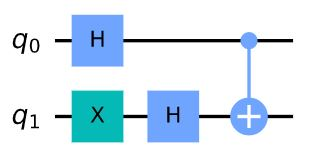
\includegraphics[width=40]{content/CNOT_HXH.JPG}
    \caption{Anwendung des CNOT-Gates auf den Qubit Zustand \(\Ket{-+}\)}

\end{figure}

\begin{align*}
    \Ket{-+}     & = \frac{1}{2}(\Ket{00} + \Ket{01} - \Ket{10} - \Ket{11})            \\
    CNOT\Ket{-+} & = \frac{1}{2}(\Ket{00} + \Ket{11} - \Ket{10} -\Ket{01}) = \Ket{--},
\end{align*}

\[\Ket{+} = Control, \quad \Ket{-} = Target.\]

\glqqDas ist interessant, weil [das CNOT-Gate] den Zustand des Control-Qubits beeinflusst, während der Zustand des Target-Qubits unverändert bleibt. [...] Kickback bedeutet, dass der durch ein Gatter zu einem Qubit hinzugefügte Eigenwert durch eine controlled-Operation in ein anderes Qubit 'zurückgekickt' wird. \grqq (ANIS u. a., 2021, Textbook ’Phase Kickback’ - Chapter 1 & 2) Dieser Effekt betrifft auch andere Controlled-Gates. \newline
\newline
Um die Funktion eines klassischen \textit{AND-Gates} zu implementieren, können verschiedene Gate-Kombinationen verwendet werden. Als Beispiel können zwei Controlled-H-Gates und ein Controlled-Z-Gate verwendet werden. Das CZ-Gate wird aus einem CNOT-Gate und zwei weiteren H-Gates gebildet. Die CH-Gates werden auf eine ähnliche Weise gebildet, jedoch werden anstelle von H-Gates jeweils Rotationen um \(\frac{\pi}{4}\) und \(-\frac{\pi}{4}\) um die Y-Achse verwendet.


\begin{figure}
    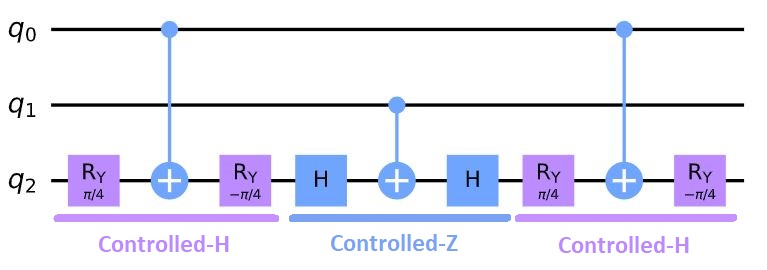
\includegraphics[width=70]{content/and-example-long.JPG}
    \caption{Beispiel Implementation eines Quantum AND-Gates aus zwei CH-Gates und einem CZ-Gate}

\end{figure}\newline


Dieses AND-Gate benötigt zwei Control-Qubits \(q_0\) und \(q_1\) sowie ein Target-Qubit \(q_2\). Bei \(\Ket{00}\) verändert sich der Zustand von \(q_2\) nicht, während unter \(\Ket{11}\) die Gatefolge \(HZH=X\), also eine NOT-Operation, auf \(q_2\) durchgeführt wird. Die Zustände \(\Ket{01}\) und \(\Ket{10}\) erzeugen entweder eine zunächst irrelevante relative Phase durch alleinige Ausführung des CZ-Gates auf \(q_2\) oder gleichen sich gegenseitig aus. \newline

Als abstrakte Betrachtung für Qubit Gates wird die Variable \(U\) verwendet, welche eine beliebige unitäre Matrix repräsentiert. Durch eine Erweiterung des CNOT-Gates kann aus dem \textit{U-Gate} ein \textit{Controlled-U-Gate} entstehen, das genau ein Control-Qubit und \(n\) Target-Qubits besitzt. Wenn das Control-Qubit im Zustand \(\Ket{0}\) ist, passiert nichts. Wenn dieses sich aber im Zustand \(\Ket{1}\) befindet, so wird auf alle \(n\) Target-Qubits das \textit{U-Gate} angewendet.

\begin{figure}
    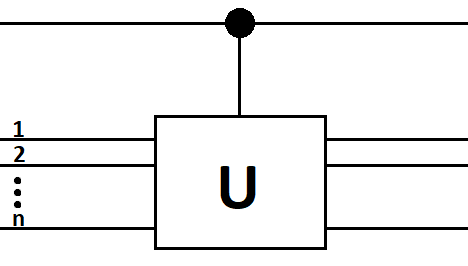
\includegraphics[width=40]{content/uGate.png}
    \caption{Controlled-U-Gate mit \(n\) Target Qubits}
\end{figure}

Mit dieser Denkweise kann beispielsweise auch das CNOT-Gate beschrieben werden: \(U=X\) und \(n=1\). (Nielsen und Chuang, 2001, Vgl. S.23)


\newline \newline
\exercise[type=multipleChoice]{
    \question{Frage: Wie funktioniert ein Controlled-NOT Gate in einem zwei Qubit System?}
    \possibleAnswers{
        \item 1) Ein Qubit übernimmt die Rolle des Controll-Qubits und das andere die des Target-Qubits. Ist das Controll-Qubit zum Zeitpunkt der Ausführung im Zustand \(\Ket{1}\), wird ein \(X\) Gate auf das Target-Qubit ausgeführt.
        \item 2) Ein Qubit übernimmt die Rolle des Controll-Qubits und das andere die des Target-Qubits. Ist das Target-Qubit zum Zeitpunkt der Ausführung im Zustand \(\Ket{1}\), wird ein \(X\) Gate auf das Controll-Qubit ausgeführt.
        \item 3) Ein Qubit übernimmt die Rolle des Controll-Qubits und das andere die des Target-Qubits. Ist das Controll-Qubit zum Zeitpunkt der Ausführung im Zustand \(\Ket{1}\), wird ein \(Z\) Gate auf das Controll-Qubit und das Target-Qubit ausgeführt.
        \item 4) Ein Qubit übernimmt die Rolle des Controll-Qubits und das andere die des Target-Qubits. Ist das Controll-Qubit zum Zeitpunkt der Ausführung im Zustand \(\Ket{0}\), wird ein \(X\) Gate auf das Controll-Qubit ausgeführt.
        \item 5) Ein Qubit übernimmt die Rolle des Controll-Qubits und das andere die des Target-Qubits. Ist das Controll-Qubit zum Zeitpunkt der Ausführung im Zustand \(\Ket{0}\), wird ein \(X\) Gate auf das Controll-Qubit und das Target-Qubit ausgeführt.
    }
    \result{1}
}


\newline \newline

\subsection{Quellen}
[ANIS u. a. 2021] Qiskit: An Open-source Framework for Quantum Computing. 2021\newline
[Nielsen und Chuang 2001] Nielsen, Michael A. ; Chuang, Isaac L.: Quantum computation and quantum information. In: Phys. Today 54 (2001), Nr. 2, S. 60\newline